\chapter{Введение}
В настоящее время радио частоты становятся все более дорогим ресурсом из-за большого количества работающих радиотехнических систем. Разумные пути для выделения радио ресурсов становятся все более и более важными в беспроводных технологиях. Методы совместного использования спектра являются одним из таких путей\cite{Book32}. Однако подобные технологии должны быть реализован очень аккуратно, для того что удерживать интерференцию на низком уровне для других легально работающих систем\cite{Book34}\cite{Book35}.  Четвертое поколение мобильной связи было основано на ОЧРК модуляции. Однако ОЧРК не предоставляло необходимого уровня межсистемной интерференции и недостаточно эффективно использовало радио ресурсы. Данный недостаток был связан с ортогональностью между всеми поднесущими частотами \cite{Book34} \cite{Book33}. В следующем поколении систем мобильной связи был предложен более эффективный путь для использования частотного ресурса. Новая техника названа Обобщенное частотное разделение каналов. Она основана на неортогональном расположении поднесущих частот. Передатчик располагает поднесущие частоты таким образом чтобы спектры данных работали с некоторым перекрытием между собой. Система обеспечивает такое поведение при помощи фильтров с характеристикой "Корень приподнятого косинуса" вместо использования согласованного фильтра. Выбранный подход позволяет уменьшить излучение вне рабочей полосы частот.Однако интерференция внутри системы значительно уменьшает производительность выбранного метода модуляции. При этом взаимное перекрытие в системе является настраиваемым параметром и таким образом система может выбирать компромисс между влиянием на чужие системы и производительностью своей системы. Так же новая система передачи данных значительно увеличивает сложность организации приемника. Это связано с тем что приемник обязан найти символы как во временной так и в частотной области.Данная задача имеет достаточно большую вычислительную сложность и увеличит размеры и энергопотребление приемного устройства. Более того для того чтобы обеспечить тот же уровень ошибок на бит приемник должен быть значительно сложнее и использовать совершенные алгоритмы расчета. При этом данную систему можно описать при помощи тензорной алгебры для того чтобы выразить ее в более естественной форме.
\section{Обработка сигналов основанная на тензорной алгебре}
Тензор это много размерный массив данных. Другими словами Н мерный тензор является матрицей у которой существуют элементы по Н разным измерениям\eqref{i_1}\cite{Book6}. Тензоры первого и второго порядка являются векторами и матрицами соответственно. Тензоры которые имеют количество измерений более двух считаются тензорами высоких порядков\cite{Book7}. 
\begin{align}
\mathcal{X} \in \compl^{I_1\times I_2\cdots I_N}
\label{i_1}
\end{align}
Порядок тензора это число измерений по которым тензор имеет различные элементы. В данной работе скалярные значения обозначены как прописные символы например $a$. Векторы обозначены как прописные символы полужирного шрифта например $\mathbf{a}$. Матрицы записаны как заглавные полужирные символы например $\mathbf{A}$. Тензоры высокого порядка обозначены как заглавные символы каллиграфического шрифта например $\mathcal{A}$. Тензоры позволяют описать данные в более естественной форме в случае если количество их естественных измерений больше двух. Описание данных при помощи тензоров позволяет учитывать многие зависимости между различными размерностями в данных. 
Развертка $N$-ого порядка является соединением тензора с фиксированной точкой одной размерности\eqref{i_2}\eqref{i_3}\eqref{i_4}\eqref{i_5}\cite{Book16}. При этом для каждого столбца все размерности за исключением одного являются фиксированными.  Развертка $N$-ого порядка имеет то же количество строк сколько имеет элементов по пространству v. Запись по столбцам может отличаться по порядку. Отличают запись по Матлаб и запись по Латауеру. Запись по Матлаб идет начиная от первого измерения к концу\cite{Book19}, в то время как по Латауеру от последнего измерения к первому. В данной работе используется запись по Матлаб во всех вычислениях, если явно не указано иное.
\begin{align}
\mathcal{X}_{:,:,1}=\begin{bmatrix}
1&3\\ 
0&1\\
\end{bmatrix} \; \mathcal{X}_{:,:,2}=\begin{bmatrix}
2&-3\\ 
-1&2\\
\end{bmatrix}
\label{i_2}
\end{align}
\begin{align}
\mathcal{X}_{[1]}=\begin{bmatrix}
1&3&2&-3\\ 
0&1&-1&2\\
\end{bmatrix}
\label{i_3}
\end{align}
\begin{align}
\mathcal{X}_{[2]}=\begin{bmatrix}
1&0&2&-1\\ 
3&1&-3&2\\
\end{bmatrix}
\label{i_4}
\end{align}
\begin{align}
\mathcal{X}_{[3]}=\begin{bmatrix}
1&0&3&1\\ 
2&-1&-3&2\\
\end{bmatrix}
\label{i_5}
\end{align}
$N$-мерный тензор имеет ранг один если он может быть представлен как внешнее произведение $N$ векторов\cite{Book6}. Разложение тензоров на тензоры ранга один было предложено Хичкоком в 1927 г\cite{Book5}. Он описал тензор высшего порядка как сумму тензоров ранга один. Тензор может быть разложен на некоторое количество тензоров ранга один. Такое разложение называют "Каноническое разложение" или "Параллельная факторизация"\eqref{i_6}\eqref{i_7}. Каноническое разложение раскладывает тензор на сумму тензоров ранга один. Данная сумма может быть представлена в иной форме.
\begin{align}
\mathcal{X}=\sum_{r=1}^R \mathbf{a}_r \circ \mathbf{b}_r \circ \mathbf{c}_r
\label{i_6}
\end{align}
\begin{align}
\mathcal{X}\in \compl^{I_1\times I_2\times I_3} \mathbf{a}_r\in \compl^{I_1\times 1} \mathbf{b}_r\in \compl^{I_2\times 1} \mathbf{c}_r\in \compl^{I_3\times 1}
\label{i_7}
\end{align} 
Векторы соответствующие тому же пространству при тензорах ранга один могут быть собраны в одну матрицу для каждой из размерностей\eqref{i_8}. Такая запись называется матричная факторизация. При помощи записанных матриц развертки каждого из порядков можно записать в значительно более простой форме\eqref{i_10}\eqref{i_11}\eqref{i_12}. 
\begin{align}
\mathcal{X}= \mathbf{A} \circ \mathbf{B} \circ \mathbf{C}
\label{i_8}
\end{align}
\begin{align}
\mathbf{A}=\begin{bmatrix}
\mathbf{a}_1&\mathbf{a}_2\cdots \mathbf{a}_R\\
\end{bmatrix}
\label{i_9}
\end{align}
\begin{align}
\mathcal{X}_{[1]}=\mathbf{A}(\mathbf{C}\diamond \mathbf{B})^T
\label{i_10}
\end{align}
\begin{align}
\mathcal{X}_{[2]}=\mathbf{B}(\mathbf{C}\diamond \mathbf{A})^T
\label{i_11}
\end{align}
\begin{align}
\mathcal{X}_{[3]}=\mathbf{C}(\mathbf{A}\diamond \mathbf{B})^T
\label{i_12}
\end{align}
Существует много путей разложить тензор, один из самых распространенных алгоритмов является метод ПМНК. Алгоритм описан ниже\cite{Book66}.
\begin{itemize}
\item Установка стартовых матриц $\mathbf{A,B,C}$ как случайных комплексных матриц фиксированного размера
\item  Решение СЛАУ с данными матрицами $\mathbf{B,C}$ и обновлением матрицы $\mathbf{A}$ 
\item Решение СЛАУ с данными матрицами $\mathbf{A,C}$ и обновлением матрицы $\mathbf{B}$ 
\item Решение СЛАУ с данными матрицами $\mathbf{A,B}$ и обновлением матрицы $\mathbf{C}$ 
\item Проверка уменьшения значения функции невязки. В случае если уменьшение больше порога, повторить с алгоритм с пункта 2.
\end{itemize}
\subsection{PARATUCK2}
Модель $PARATUCK2 $\cite{Book12} является комбинацией между $PARAFAC $\cite{Book6} и $TUCKER3$\cite{Book6} моделями разложения тензоров. Модель позволяет разложить один трехмерный тензор на 5 различных матриц. В общем случае модель может быть записана в скалярной форме при помощи следующего выражения\eqref{p_1} \cite{Book26}. 
\begin{align}
x_{i_1,i_2,t}=\sum^{F}_{f=1} \sum^{T_s}_{t_s=1}a_{i_1,f}c^{[a]}_{t,f}s_{f,t_s}c^{[b]}_{f,t_s}b_{i_2,t_s}
\label{p_1}
\end{align}
\begin{align*}
\mathcal{X} \in \compl^{I_1 \times, I_2 \times T} \mathbf{A} \in \compl^{I_1 \times F} \mathbf{B} \in \compl^{I_2 \times T_s}
\end{align*}
\begin{align*}
\mathbf{C}^{[a]} \in \compl^{T \times F} \mathbf{C}^{[b]} \in \compl^{T \times T_s}
\end{align*}
В указанном выше выражении $x_{i_1,i_2,t}$  является $(i_1,i_2,t)$  элементом тензора $\mathcal{X} \in \compl^{I_1 \times I_2 \times T }$. Матрица $\mathbf{S}$ является  матрицей-основой для $PARATUCK2$ модели. Матрицы $\mathbf{A}$ и $\mathbf{B}$ обеспечивают связь между соответствующей размерностью тензора $\mathcal{X}$ и  матрицы-основы $\mathbf{S}$\cite{Book12}. Матрицы $\Camat$ и $\Cbmat$ являются взвешивающими коэффициентами для матриц $\Amat$ и $\Bmat$ в каждом из слоев третьей размерности тензора $\Xiten$. 
Модель может быть записана в двух формах: послойная тензорная нотация\eqref{p_2} и векторизованная форма для тензора $\Xiten$.
В послойной форме записи тензор $\Xiten$ записывается отдельным выражением для каждого слоя третьей размерности.  Подобная запись позволяет описать модель при помощи линейной алгебры с минимальными изменениями в выражении для различных слоев. Матрицы $\Camat$ и $\Cbmat$ в таком случае записаны как тензор с элементами на главной диагонали между первым и вторым измерением. В таком случае послойная запись для модели $PARATUCK2 $ может быть выражена как послойное произведение между матрицей $\Amat$ и $\Bmat$ с коэффициентам для соответствующих строк и столбцов для матрицы$\Camat$ и $\Cbmat$ для соответствующего слоя третьего измерения\cite{Book12}.
\begin{align}
\mathbf{X}_{:,:,i}=\mathbf{A}\cdot diag(\mathbf{C^{[a]}}_{:,i})\cdot \mathbf{S}\cdot diag(\mathbf{C^{[b]}}_{:,i})\cdot \mathbf{B}
\label{p_2}
\end{align}
Векторизованная форма тензора $\Xiten$ является второй формой для записи модели. Возможно использовать данную запись в трех формах\cite{Book6}, в виде произведения матрицы с векторизованной матрицей $\Amat$ $\Bmat$ и $\mathbf{S}$. Таким образом можно найти каждую из матриц $\Amat$ $\Bmat$ и $\mathbf{S}$ используя векторизованную модель тензора $\Xiten$ и генерирующую матрицу для каждой из форм записи. Однако важно заметить, что векторизированная модель требует знания размерностей тензора $\Xiten$ так как вектор не позволяет узнать соответствующие размерности\cite{Book5}.
\begin{align}
vec(\mathcal{X})=\begin{bmatrix}
(\mathbf{C^{[a]T}} \diamond \mathbf{C^{[b]T}})^T \diamond (vec(A_{1,:})\otimes B)\\
(\mathbf{C^{[a]T}} \diamond \mathbf{C^{[b]T}})^T \diamond (vec(\mathbf{A}_{2,:})\otimes \mathbf{B})\\
\vdots \\
(\mathbf{C^{[a]T}} \diamond \mathbf{C^{[b]T}})^T \diamond (vec(\mathbf{A}_{I_1,:})\otimes \mathbf{B})\\
\end{bmatrix} vec(\mathbf{S})
\label{p_3}
\end{align}
\begin{align}
vec(\mathcal{X})=(\mathbf{I} \otimes(((\mathbf{B}\diamond \mathbf{C}^{[b]}) \cdot \mathbf{S}^T) \odot \mathbf{C}^{[a]}) )vec(\mathbf{A})
\label{p_4}
\end{align}
\begin{align}
vec(\mathcal{X})=(\mathbf{I} \otimes (((\mathbf{A}\diamond \mathbf{C}^{[a]}) \cdot \mathbf{S}) \odot \mathbf{C}^{[b]} ))vec(\mathbf{B})
\label{p_5}
\end{align}
Векторизированная модель записи может быть упрощена в случае если матрица $\Amat$ и матрица $\Bmat$ являются векторами,а не матрицами. В данном случае модель выраженная при помощи произведений Хатри-Рао и Адамара упрощаются до значительно меньшего количества операций, и произведение Кронекера исключается.
Упрощенная форма записывается для всех трех матриц в следующей форме.
\begin{align}
vec(\mathcal{X})^T=\mathbf{a}\cdot (\mathbf{C}^{[a]T} \odot (\mathbf{S}\cdot (\mathbf{C}^{[b]}\diamond \mathbf{b}^T)^T))
\label{p_6}
\end{align}
\begin{align}
vec(\mathcal{X})^T=\mathbf{b}^T\cdot (\mathbf{C}^{[b]T} \odot (\mathbf{S}^T  \cdot (\mathbf{C}^{[a]}\diamond \mathbf{a})^T))
\label{p_7}
\end{align}
\begin{align}
vec(\mathcal{X})=(((\mathbf{a}\diamond \mathbf{C}^{[a]}) \cdot \mathbf{S}) \odot \mathbf{C}^{[b]} )\mathbf{b})
\label{p_8}
\end{align}
\begin{align}
vec(\mathcal{X})=(((\mathbf{b}^T\diamond \mathbf{C}^{[b]}) \cdot \mathbf{S}^T) \odot \mathbf{C}^{[a]}) \mathbf{a}^T) 
\label{p_9}
\end{align}
\begin{align*}
\mathcal{X} \in \compl^{1 \times 1 \times T} 
\mathbf{a} \in \compl^{1 \times F} 
\mathbf{b} \in \compl^{T_s \times 1}
\end{align*}
\begin{align*}
\mathbf{C}^{[a]} \in \compl^{T \times F}
\mathbf{C}^{[b]} \in \compl^{T \times T_s}
\mathbf{S} \in \compl^{F \times T_s}
\end{align*}
Модель будет использована для описания выраженной ниже системы модуляции ОбЧРК. Данная модель позволяет описать систему передачи данных в достаточно простой форме. 
\section{Обобщенное частотное разделение каналов}
Основной принцип работы ОбЧРК является организация блока передачи в котором используется несколько поднесущих и несколько символов на каждой из поднесущих. При этом символы на поднесущих проходят низкочастотную фильтрацию для уменьшения межканальной интерференции. В системах с обобщенное частотное разделение каналов используется два основных вида фильтров во временной области: фильтр с характеристикой "Приподнятый косинус" либо фильтр с характеристикой корень приподнятого косинуса. В системе ортогонального частотного разделения каналов используется согласованный фильтр, обеспечивающий ортогональность различных поднесущих. В системах передачи данных с ОбЧРК поднесущие не ортогональны друг другу. По этой причине возникает наложение различных поднесущих друг на друга, что увеличивает меж символьную и меж канальную интерференцию. Однако подобный подход позволяет плотнее располагать поднесущие между собой и эффективнее использовать спектр.
\subsection{Принцип конструирования низкочастотного фильтра}
Как было сказано выше в ОбЧРК используется два основных вида фильтров во временной области: фильтр с характеристикой "Приподнятый косинус" либо фильтр с характеристикой корень приподнятого косинуса. Оба фильтра имеют одну переменную значение которой можно изменять для изменения перекрытия в частотной области между каналами $\alpha$. При этом значению переменной $\alpha=0$ соответствует минимальное перекрытие между соседними поднесущими, в то время как при значении $\alpha=1$ перекрытие является максимальным. При увеличении $\alpha$ значительно увеличивается меж-символьная и меж-канальная интерференция. В системе ОбЧРК происходит усложнение структуры приемника по сравнению с ОЧРК. Приемник должен обеспечивать прием даже в условиях меж-канальной интерференции и иметь механизмы для ее устранения.
Фильтр с характеристикой "Приподнятый косинус" является усовершенствованием согласованного фильтра, его характеристики широко освещены в литературе. Выражение для импульсной характеристики представлено в \eqref{g_1} и взято из источника \cite{Book17}. В выражении переменная $T$ является длительностью одного символа в шкале временных отсчетов, $\alpha$ как и было описано является переменной. Импульсная характеристика для для различных величин $\alpha$ представлена на рис. Соответствующая частотная характеристика для величин $\alpha$ представлена на рис. 
\begin{align}
\begin{matrix}
h(t)&=&\left\{
\begin{matrix}
\frac{\pi sinc(\frac{1}{2\alpha})}{4}& t=\pm \frac{T}{2\alpha}\\
sinc(1/T)\frac{cos(\pi \alpha t/T)}{1-(2 \alpha t /T)^2}&otherwise\\
\end{matrix} \right.
\end{matrix}
\label{g_1}
\end{align}
\begin{figure}[H]
\centering
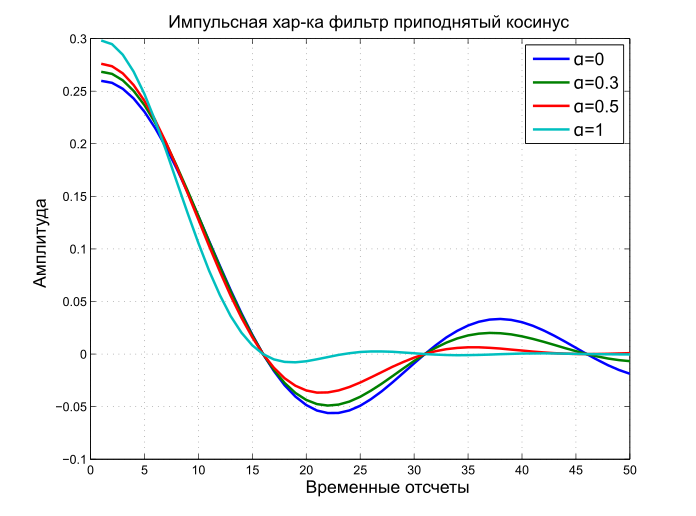
\includegraphics[width=0.9\columnwidth]{RC_time.png}
\caption{\textit{Импульсная характеристика фильтра типа Приподнятый косинус в зависимости от коэффициента $\alpha$}}
\label{fg_1}
\end{figure}
\begin{figure}[H]
\centering
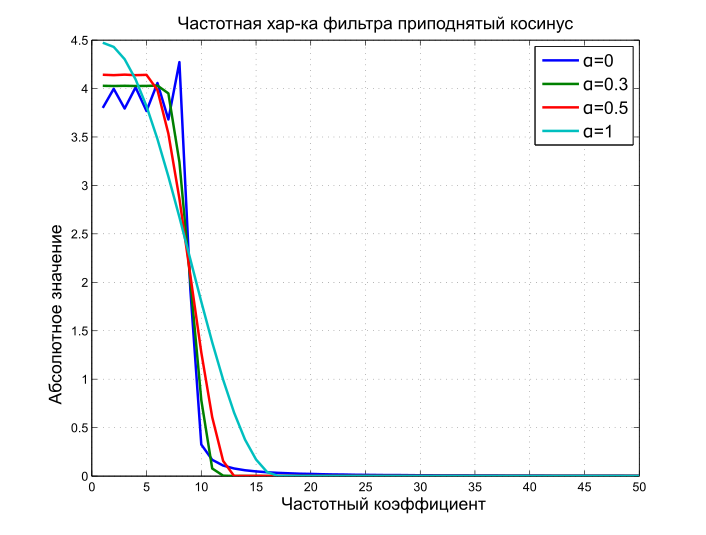
\includegraphics[width=0.9\columnwidth]{RC_freq.png}
\caption{\textit{Частотная характеристика фильтра Приподнятый косинус в зависимости от коэффициента $\alpha$}} 
\label{fg_2}
\end{figure}
Фильтр с характеристкой корень из приподнятого косинуса является дополнением к фильтру с характеристикой приподнятый косинус и при применении на приемнике и передатчике одновременно обеспечивает аналогичный уровень  межсимвольной интерференции как в согласованном фильтре. Описание и теоретическое обоснование использование фильтра описано в \cite{Book23} \cite{Book44} и \cite{Book51}. Выражение для импульсной характеристики представлено в \eqref{g_2} и взято из источника \cite{Book23}. В выражении переменная $T$ является длительностью одного символа в шкале временных отсчетов, $\alpha$ как и было описано является переменной. Импульсная характеристика для для различных величин $\alpha$ представлена на рис. Соответствующая частотная характеристика для величин $\alpha$ представлена на рис \eqref{fg_3}. 
\begin{figure}[H]
\centering
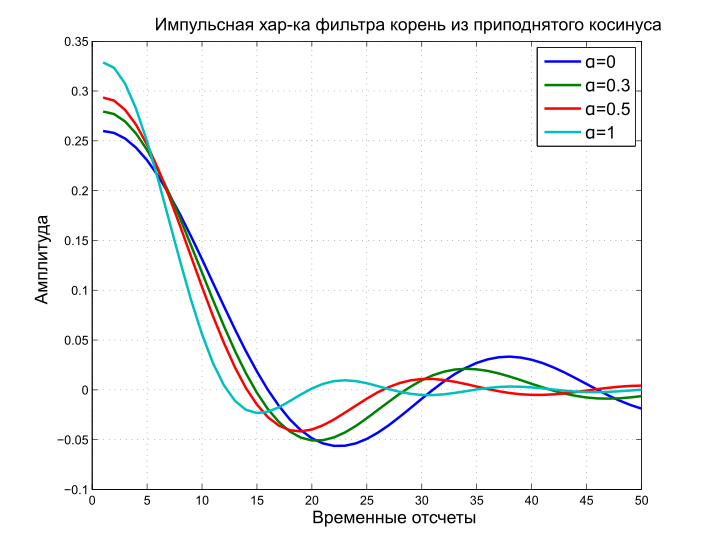
\includegraphics[width=0.9\columnwidth]{RRC_time.png}
\caption{\textit{Импульсная характеристика фильтра типа корень из Приподнятого косинуса в зависимости от коэффициента $\alpha$}} \label{fg_3}
\end{figure}
\begin{figure}[H]
\centering
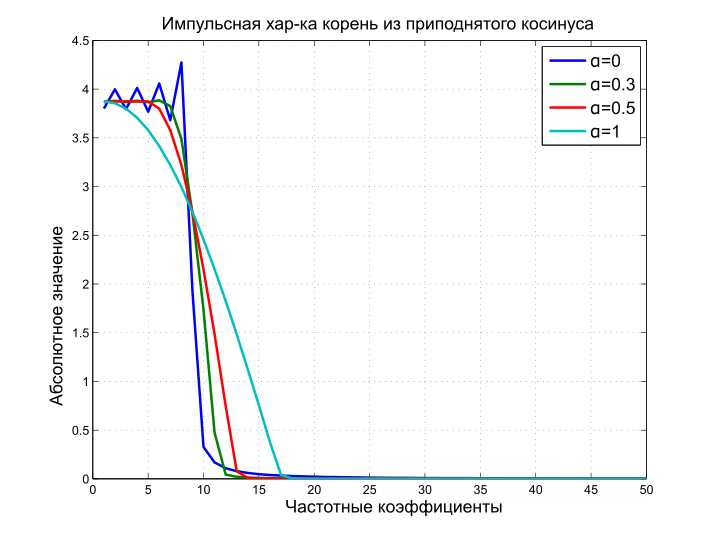
\includegraphics[width=0.9\columnwidth]{RRC_freq.png}
\caption{\textit{Частотная характеристика фильтра корень из Приподнятого косинуса в зависимости от коэффициента $\alpha$}} \label{fg_4}
\end{figure}
\begin{align}
\begin{matrix}
h(t) &=& \left\{ \begin{matrix} 
\frac{1-\alpha +4\alpha/\pi}{\sqrt{T}}& if& t=0\\
\frac{\alpha}{\sqrt{2T}}[(1+\frac{2}{\pi})sin(\frac{\pi}{4\alpha})+(1-\frac{2}{\pi})cos(\frac{\pi}{4\alpha})] & if &t= \pm T/4\alpha\\
\frac{1}{\frac{t\pi}{\sqrt{T}}(1-\frac{4*\alpha t}{T})^2}(sin(\frac{\pi t (1-\alpha)}{T})+\frac{4\alpha t}{T} cos(\frac{\pi t (1+ \alpha)}{T}) ) &otherwise \\
\end{matrix} \right.
\end{matrix}
\label{g_2}
\end{align}
Сравнение импульсных характеристик для согласованного фильтра, фильтра "Приподнятый косинус" и фильтра корень из приподнятого косинуса представлено на рис. Из рис.\eqref{fg_5} видно, что в точке где временной отсчет равен длительности импульса для согласованного фильтра амплитуда импульсной характеристики равна нулю, в отличие от других фильтров. Сравнение частотных характеристик для согласованного фильтра, фильтра "Приподнятый косинус" и фильтра корень из приподнятого косинуса представлено на рис. Из рис. видно, что для фильтра с характеристикой корень из приподнятого косинуса перекрытие по частоте является наибольшим в отличие от согласованного фильтра и фильтра с приподнятым косинусом.
\begin{figure}[H]
\centering
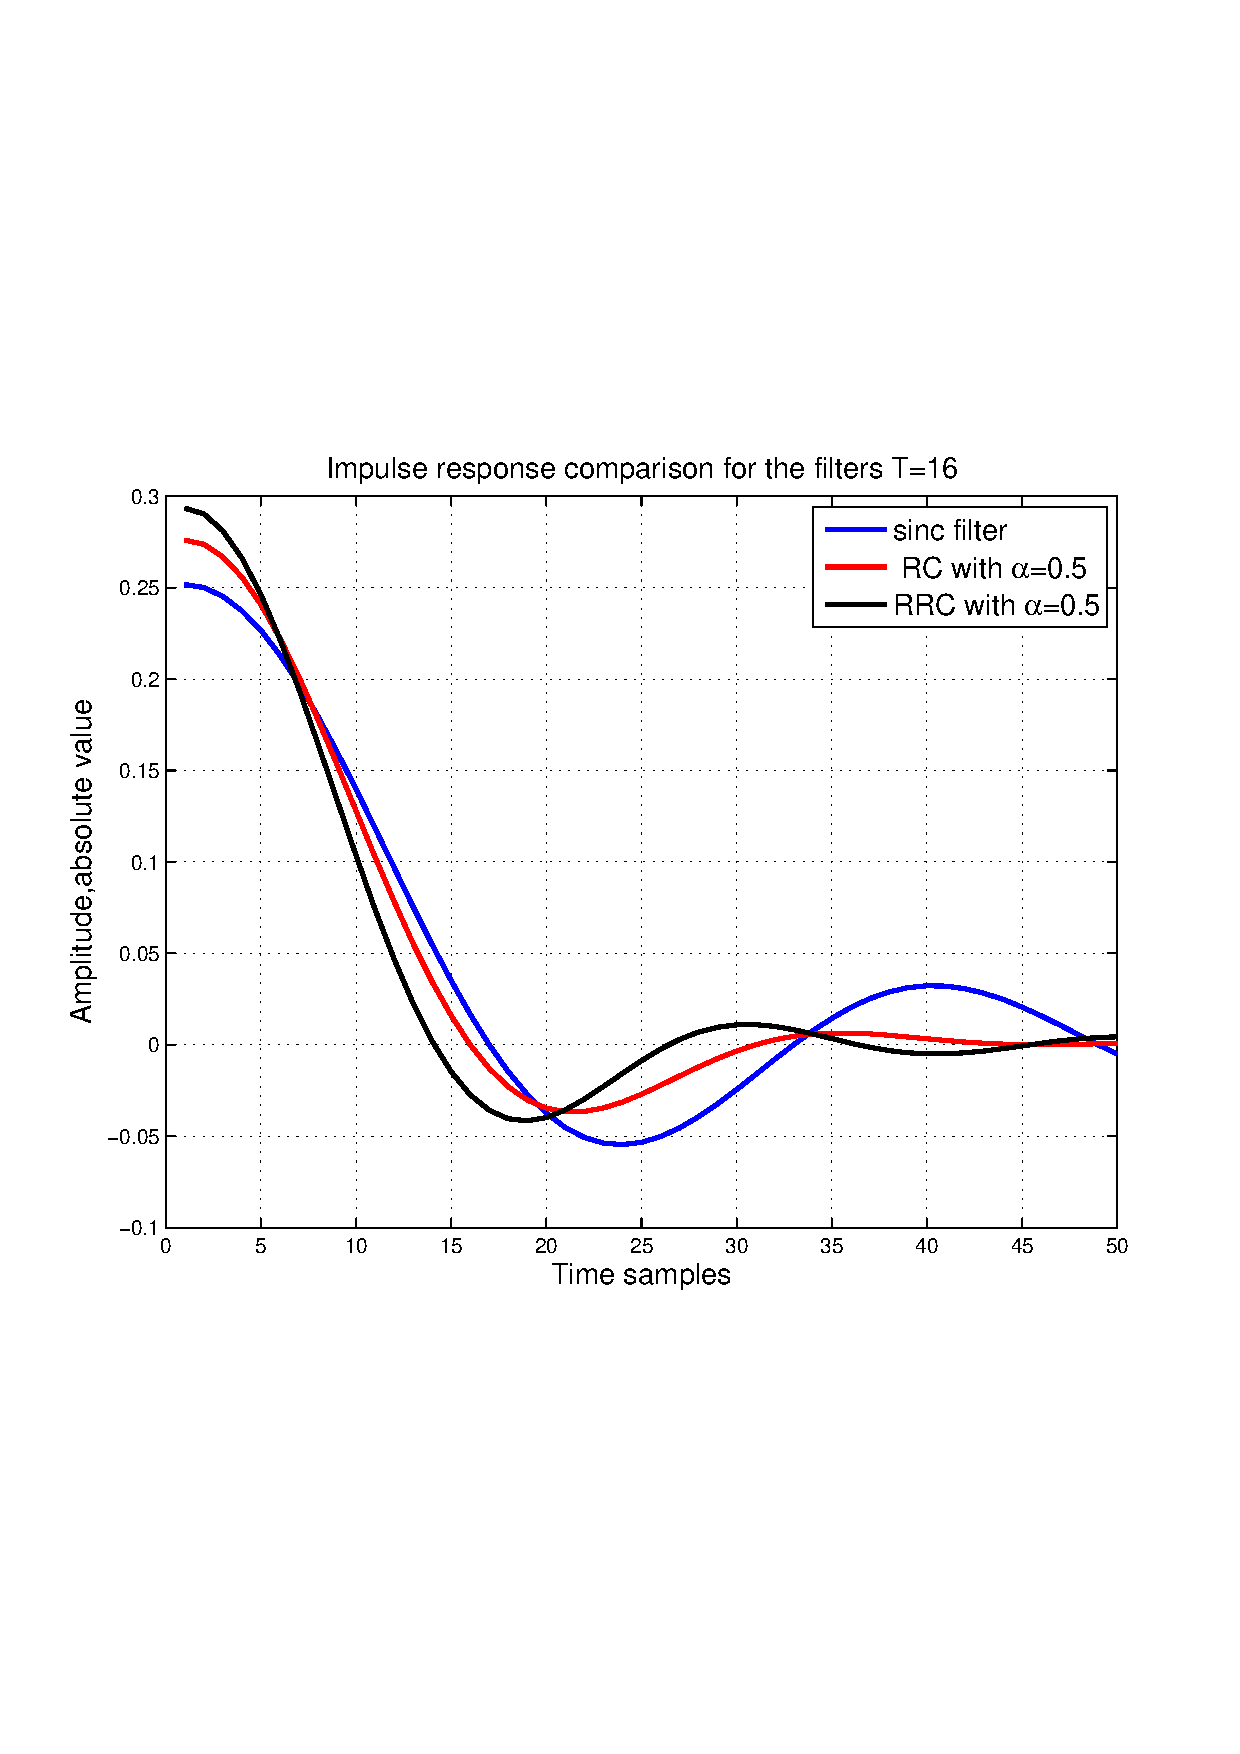
\includegraphics[width=0.9\columnwidth]{TIME_comp.png}
\caption{\textit{Сравнение импулсьных характеристик различных фильтров}} \label{fg_5}
\end{figure}
\begin{figure}[H]
\centering
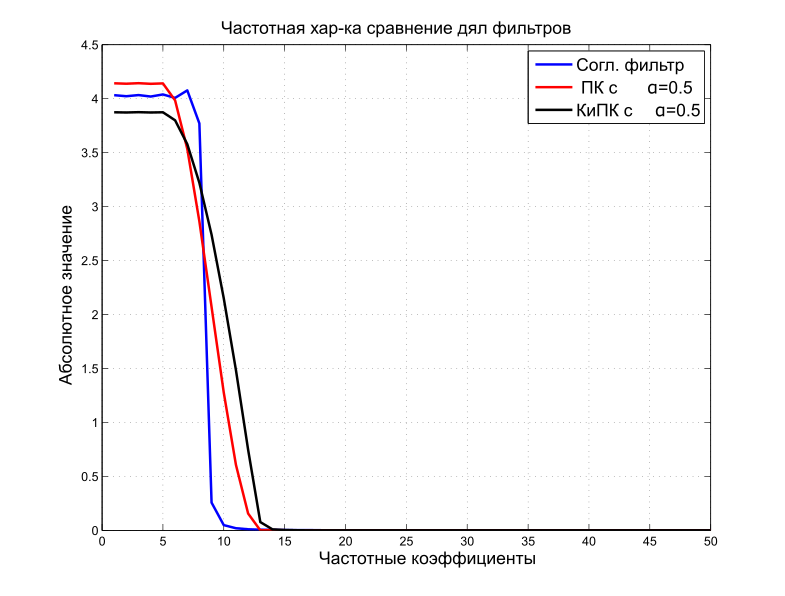
\includegraphics[width=0.9\columnwidth]{FREQ_comp.png}
\caption{\textit{С}} \label{fg_6}
\end{figure}
\section{Итеративный алгоритм с мягким порогом}
Одна из наиболее часто решаемых задач является задача деконволюции\cite{}. В матричной форме данная задача записывается как решение системы линейных алгебраических уравнений. Однако основной трудностью в решении СЛАУ является число обусловленности генерирующей матрицы\cite{Book66}. Увеличение числа обусловленности матрицы уменьшает стабильность решения СЛАУ. При этом число обусловленности является мультипликативным коэффициентом при погрешности вычисления\cite{Book55}. В классической постановке задача представлена на выражении \eqref{Book51} и может быть расписана следующим образом \eqref{ista_1}\cite{Book49}.
\begin{align}
R(x)=\mid\mid\mathbf{y}-\mathbf{Ax}\mid\mid^2_2 
\label{ista_1}
\end{align}
\begin{align}
R(x)=(\mathbf{y}-\mathbf{Ax})^H(\mathbf{y}-\mathbf{Ax})
\label{ista_2}
\end{align}
 В большинстве случаев для решения данной задачи используется обратная или псевдообратная матрица. В статье \cite{Book27} представлен итеративный алгоритм обеспечивающий сходимость к решению. При этом алгоритм гарантирует уменьшение функции невязки на каждой итерации. Основой и используемого алгоритма является "максимизация-минимизация". Подход позволяет заменить одну сложную задачу большим количеством простых задач. Каждая оптимизационная задача обеспечивает решение которое будет  находится ближе к решению задачи. На каждой итерации к исходной проблеме добавляется не отрицательное дополнительное слагаемое. Слагаемое должно быть таким, чтобы решаемая задача на данной итерации стала проще\cite{Book26}. Так же есть некоторые требования для дополнительного слагаемого $J_{add}(\mathbf{x})$ . Функция $J_{add}(\mathbf{x})$ должна удовлетворять выражению  $J_{add}(\mathbf{x})\geq R(\mathbf{x})$ для всех $\mathbf{x}$  и более того в точке $\mathbf{x}_k$ соответствующей текущему решению должно выполняться условие $J_{add}(\mathbf{x_k})= R(\mathbf{x_k})$.  Функциям $J_{add}(\mathbf{x})$ может быть различной на каждой итерации и должна обеспечивать простую минимизацию. Описанный ниже метод удовлетворяющий всем условиям назван "итерация  Ланвебера"\cite{Book24}. В оригинальной форме алгоритм написан для задач с действительными числами однако его можно расширить и для комплексных чисел. Определим $1$ как функция записанную в \eqref{ista_3}. В таком случае оптимизируемая функция будет записана в следующей форме $ R_1(\mathbf{x})$ \eqref{Book28} где $\alpha$ является коэффициентом для которого должно выполняться условие \eqref{ista_5}. Перепишем выражение раскрыв скобки и упростим его.
 
 \begin{align}
 \alpha \geq max(eig(\mathbf{A^HA}))
 \end{align}
 \begin{align}
 R(\mathbf{x_{k+1}})<R(\mathbf{x_k})
 \label{ista_3}
 \end{align}
\begin{align}
 R_1(\mathbf{x})=R(\mathbf{x})+J_{add}(\mathbf{x}) \label{ista_4}
\end{align}
\begin{align}
 R_1(\mathbf{x})=\mid\mid\mathbf{y}-\mathbf{Ax}\mid\mid^2_2+J_{add}(\mathbf{x})\label{ista_5}
\end{align}
\begin{align}
J_{add}(\mathbf{x})=(\mathbf{x-x_k})^T(\alpha \mathbf{I}-\mathbf{A}^T\mathbf{A})(\mathbf{x-x_k})\label{ista_6}
\end{align}
\begin{align}
 R_1(\mathbf{x})=\mid\mid\mathbf{y}-\mathbf{Ax}\mid\mid^2_2+(\mathbf{x-x_k})^H(\alpha \mathbf{I}-\mathbf{A}^H\mathbf{A})(\mathbf{x-x_k}) \label{ista_7}
\end{align}
\begin{align}
 R_1(\mathbf{x})=(\mathbf{y}-\mathbf{Ax})^H(\mathbf{y}-\mathbf{Ax})+(\mathbf{x}-\mathbf{x}_k)^H(\alpha \mathbf{I}-\mathbf{A}^H\mathbf{A})(\mathbf{x}-\mathbf{x}_k) \label{ista_8}
\end{align}
\begin{align}
\alpha \geq max(eig(\mathbf{A}^H\mathbf{A})) \label{ista_9}
\end{align}
\begin{align}
R_1(\mathbf{x})=\mathbf{y}^H\mathbf{y} -\mathbf{y}^H\mathbf{A}\mathbf{x} -\mathbf{x}^H \mathbf{A}^H\mathbf{y} +\mathbf{x}^H\mathbf{A}^H\mathbf{A}\mathbf{x} \label{ista_10}
\end{align}
\begin{align*}
 +\mathbf{x}_k^H(\alpha \mathbf{I}-\mathbf{A}^H\mathbf{A})\mathbf{x}_k +\mathbf{x}^H(\alpha \mathbf{I}-\mathbf{A}^H\mathbf{A})\mathbf{x} 
\end{align*}
\begin{align*}
-\mathbf{x}_k^H(\alpha \mathbf{I}-\mathbf{A}^H\mathbf{A})\mathbf{x} -\mathbf{x}^H(\alpha \mathbf{I}-\mathbf{A}^H\mathbf{A})\mathbf{x}_k 
\end{align*}
Описанная функция $ R_1(\mathbf{x})$ является вогнутой. Вогнутая функция имеет производную равную нулю в одной точке и эта точка является точкой минимума. Таким образом для нахождения точки минимума необходимо приравнять производную оптимизируемой функции к нулю и найти решение полученного уравнения. Поскольку функция является комплексной, она не аналитичная и от нее не существует аналитической производной. Для нахождения производной мы использовали  исчисление Виртингера\cite{Book27} и нашли производную по комплексно-сопряженной к искомой величине. В дальнейшем при упрощении выражения мы получаем в явном виде формулу для перехода от итерации к итерации \eqref{ista_11} позволяющую в конечном итоге привести производную оптимизируемой функции к нулю. Описанный алгоритм позволяет достичь линейной сходимости переменной $\mathbf{x}_k$, а так же уменьшить вычислительные затраты на работу алгоритма\cite{Book24}. 
\begin{align}
\frac{\delta R_1(x)}{\delta x^*}=-\mathbf{A}^H\mathbf{y} +\mathbf{A}^H\mathbf{A}\mathbf{x} +(\alpha \mathbf{I}-\mathbf{A}^H\mathbf{A})\mathbf{x} -(\alpha \mathbf{I}-\mathbf{A}^H\mathbf{A})\mathbf{x}_k \label{ista_11}
\end{align}
\begin{align}
\frac{\delta R_1(x)}{\delta x^*}=-\mathbf{A}^H\mathbf{y} +\alpha\mathbf{x} -\alpha\mathbf{x}_k+\mathbf{A}^H\mathbf{A}\mathbf{x}_k=0 \label{ista_12}
\end{align}
\begin{align}
\mathbf{A}^H(\mathbf{y} -\mathbf{A}\mathbf{x}_k) +\alpha\mathbf{x}_k =\alpha\mathbf{x} \label{ista_13}
\end{align}
\begin{align}
\mathbf{x}=\frac{\mathbf{A}^H}{\alpha}(\mathbf{y} -\mathbf{A}\mathbf{x}_k) +\mathbf{x}_k \label{ista_14}
\end{align}
\begin{align}
\mathbf{x}_{k+1}=\frac{\mathbf{A}^H}{\alpha}(\mathbf{y} -\mathbf{A}\mathbf{x}_k) +\mathbf{x}_k \label{ista_15}
\end{align}
К описанному алгоритму существует усовершенствование позволяющее достичь квадратичной сходимости без значительного увеличения вычислительной стоимости. Кроме того модификация описанного алгоритма позволяет решать задачу сжатого считывания путем использования мягкого порога около нулевого значения\cite{Book28}.
\begin{itemize}
\item Установить начальную точку $\mathbf{x}_0$ и установить промежуточные переменные $t_0=1, t_1=1$
\item Установить $\mathbf{y}_1=\mathbf{x}_0$
\item Обновить значение $t_1$ при помощи выражения \eqref{ista_16}
\item Найти решение выражение \eqref{ista_17} для итерации 
\item Установить $t_0=t_1$
\item Обновить промежуточную переменную при помощи выражения \eqref{}
\item Проверить, если величина шага на итерации меньше чем заданный порог. Если шаг больше, повторить операция с шага 3
\end{itemize}
\begin{align}
t_1=\frac{1+\sqrt{1+4t_1}}{2} \label{ista_16}
\end{align}
\begin{align}
\mathbf{x}_{k+1}=\frac{\mathbf{A}^H}{\alpha}(\mathbf{Y} -\mathbf{A}\mathbf{x}_k) +\mathbf{x}_k+\frac{t_0-1}{t_1}\cdot (\mathbf{x}_k-\mathbf{x}_{k-1}) \label{ista_17}
\end{align}
\clearpage